% A '%' character causes TeX to ignore all remaining text on the line,
% and is used for comments like this one.

\documentclass{article}      % Specifies the document class
\usepackage{amsmath, nccmath}
\usepackage{enumitem}
\usepackage{graphicx}
\usepackage[utf8]{inputenc}
\usepackage{listings}
\usepackage{xcolor}
\usepackage{float}
\graphicspath{ {./} }
\definecolor{codegreen}{rgb}{0,0.6,0}
\definecolor{codegray}{rgb}{0.5,0.5,0.5}
\definecolor{codepurple}{rgb}{0.58,0,0.82}
\definecolor{backcolour}{rgb}{0.95,0.95,0.92}

\lstdefinestyle{mystyle}{
    backgroundcolor=\color{backcolour},   
    commentstyle=\color{codegreen},
    keywordstyle=\color{magenta},
    numberstyle=\tiny\color{codegray},
    stringstyle=\color{codepurple},
    basicstyle=\ttfamily\footnotesize,
    breakatwhitespace=false,         
    breaklines=true,                 
    captionpos=b,                    
    keepspaces=true,                 
    numbers=left,                    
    numbersep=5pt,                  
    showspaces=false,                
    showstringspaces=false,
    showtabs=false,                  
    tabsize=2
}

\lstset{ 
    language=Python, % choose the language of the code
    basicstyle=\fontfamily{pcr}\selectfont\footnotesize\color{red},
    keywordstyle=\color{black}\bfseries, % style for keywords
    numbers=none, % where to put the line-numbers
    numberstyle=\tiny, % the size of the fonts that are used for the line-numbers     
    backgroundcolor=\color{darkgray},
    showspaces=false, % show spaces adding particular underscores
    showstringspaces=false, % underline spaces within strings
    showtabs=false, % show tabs within strings adding particular underscores
    frame=single, % adds a frame around the code
    tabsize=2, % sets default tabsize to 2 spaces
    rulesepcolor=\color{gray},
    rulecolor=\color{black},
    captionpos=b, % sets the caption-position to bottom
    breaklines=true, % sets automatic line breaking
    breakatwhitespace=false, 
}

\lstset{style=mystyle}


\title{CEE 498 Applied Machine Learning - HW6 }  % Declares the document's title.
\author{Rini Jasmine Gladstone (rjg7) and Maksymilian Podraza (podraza3)}      % Declares the author's name.
\date{May 7 2020}      % Deleting this command produces today's date.

\newcommand{\ip}[2]{(#1, #2)}
                             % Defines \ip{arg1}{arg2} to mean
                             % (arg1, arg2).

%\newcommand{\ip}[2]{\langle #1 | #2\rangle}
                             % This is an alternative definition of
                             % \ip that is commented out.

\begin{document}             % End of preamble and beginning of text.

\maketitle                   % Produces the title.


\section{Problem 1}      % Produces section heading.  Lower-level
                             % sections are begun with similar 
                             % \subsection and \subsubsection commands.

We built  a linear regression of the log of the concentration against the log of time. 
\begin{figure}[H]
\centering
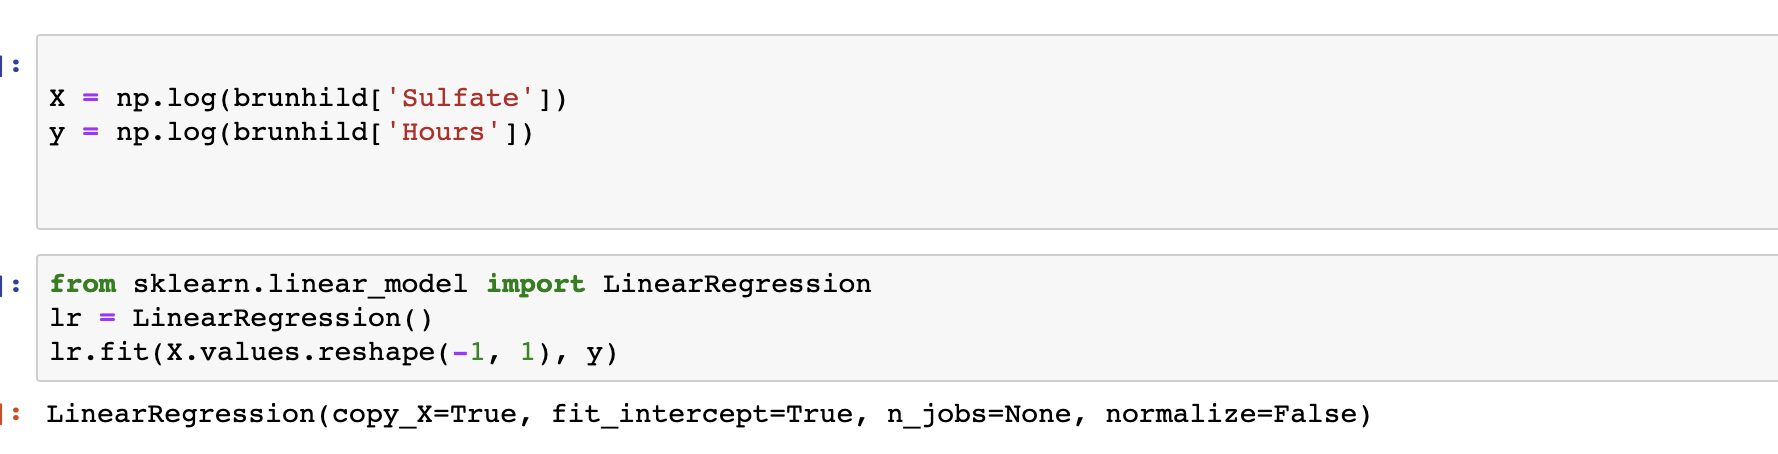
\includegraphics[width=\textwidth]{part1}
\end{figure}

\subsection{Part a} Please find below the plot showing the data points and the regression line in log-log coordinates

\begin{figure}[H]
\centering
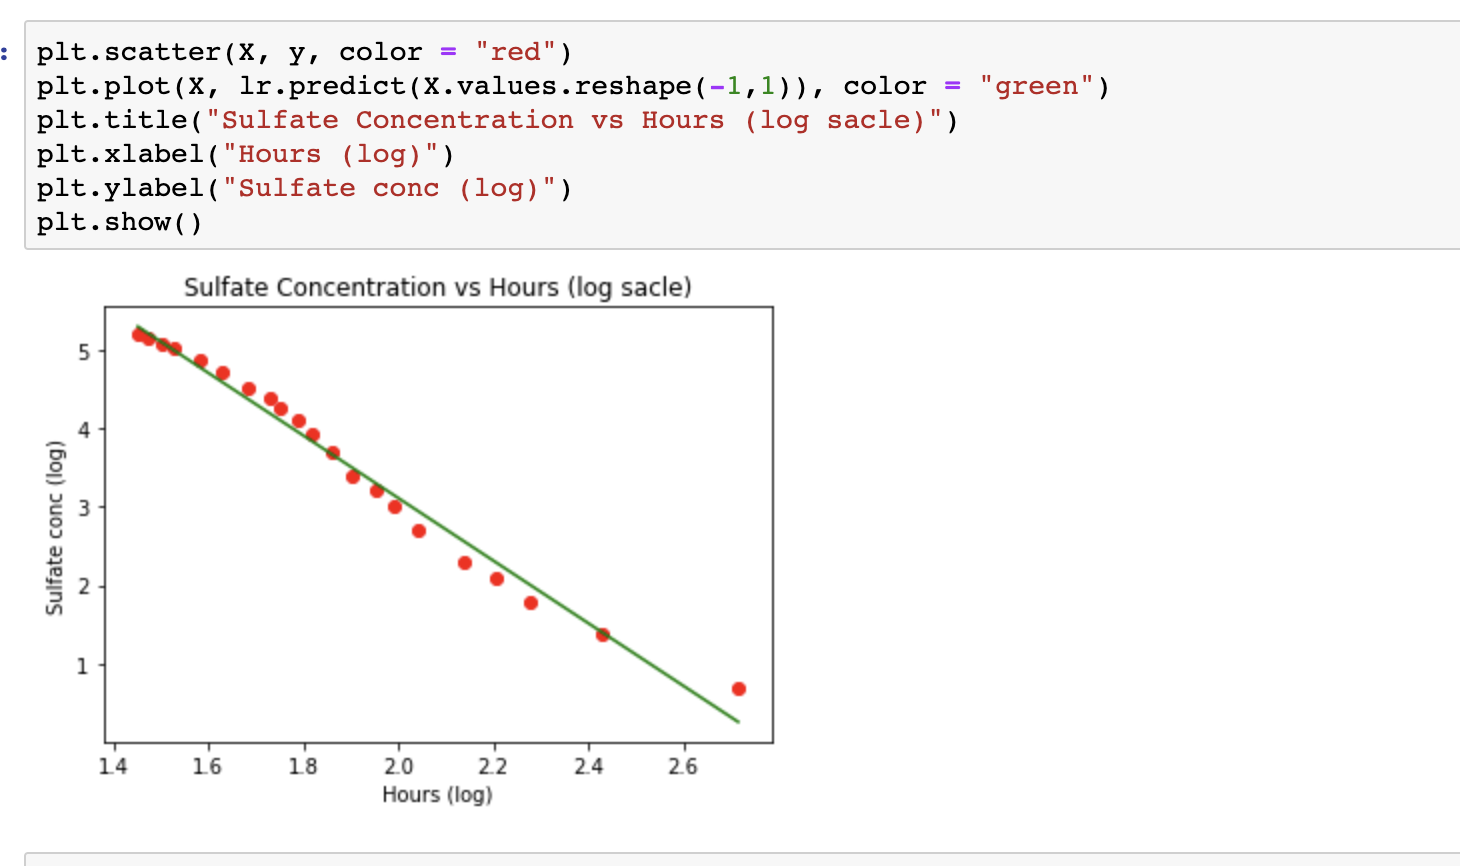
\includegraphics[width=\textwidth]{part2}
\end{figure}

\subsection{Part b} Please find below the plot showing the data points and the regression line in original coordinates

\begin{figure}[H]
\centering
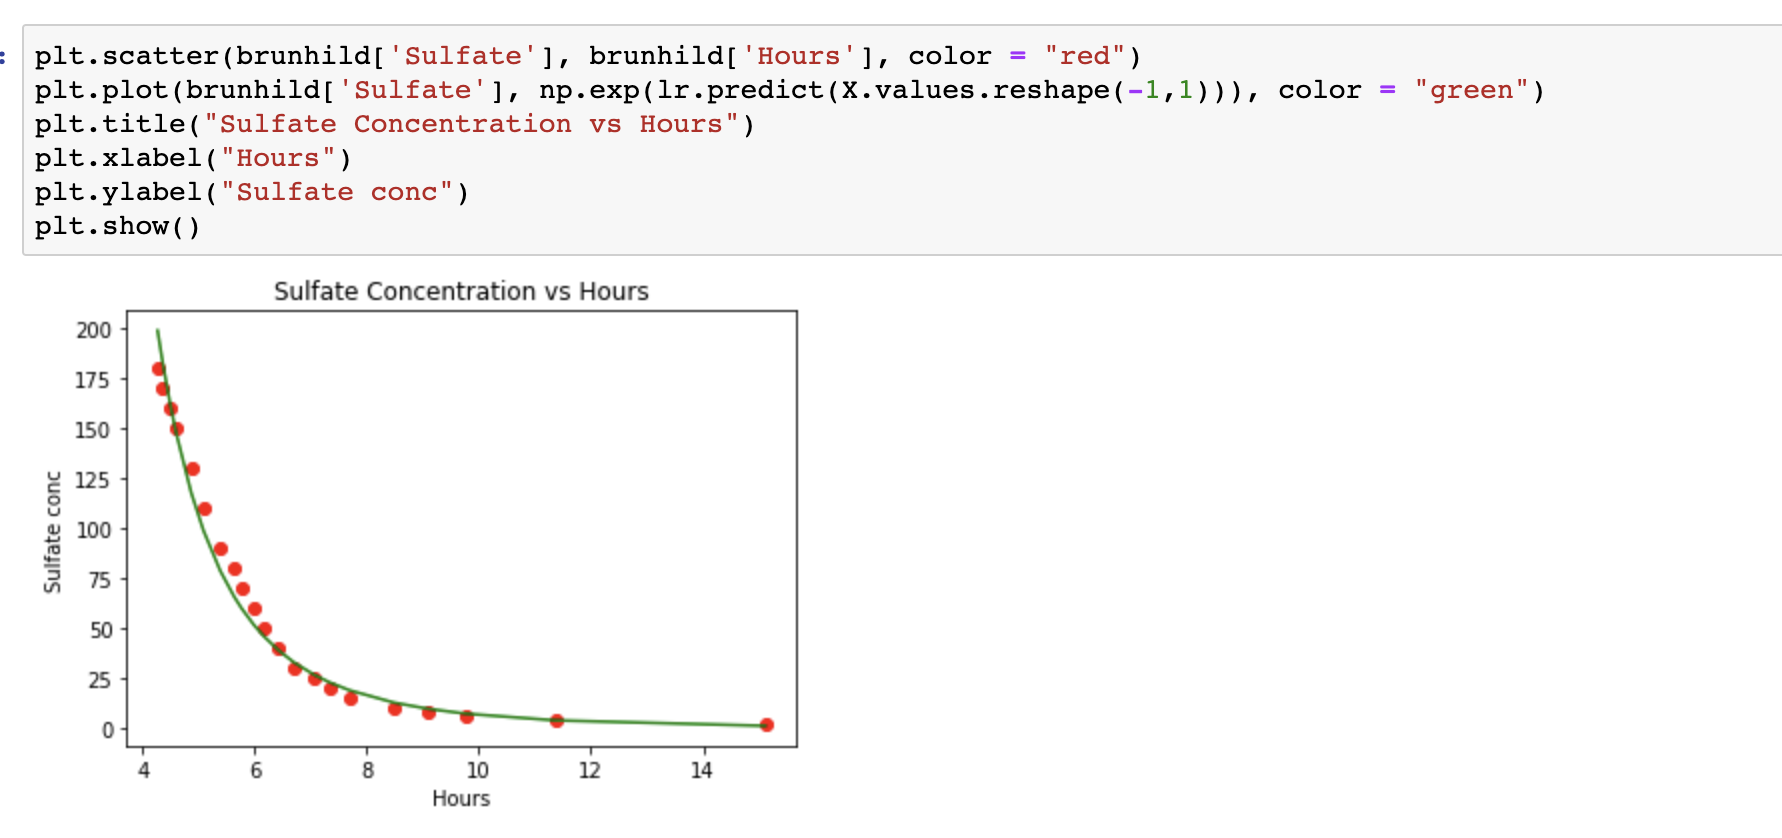
\includegraphics[width=\textwidth]{part3}
\end{figure}

\subsection{Part c} Please find below the plot showing the residual against the fitted values in log-log coordinates

\begin{figure}[H]
\centering
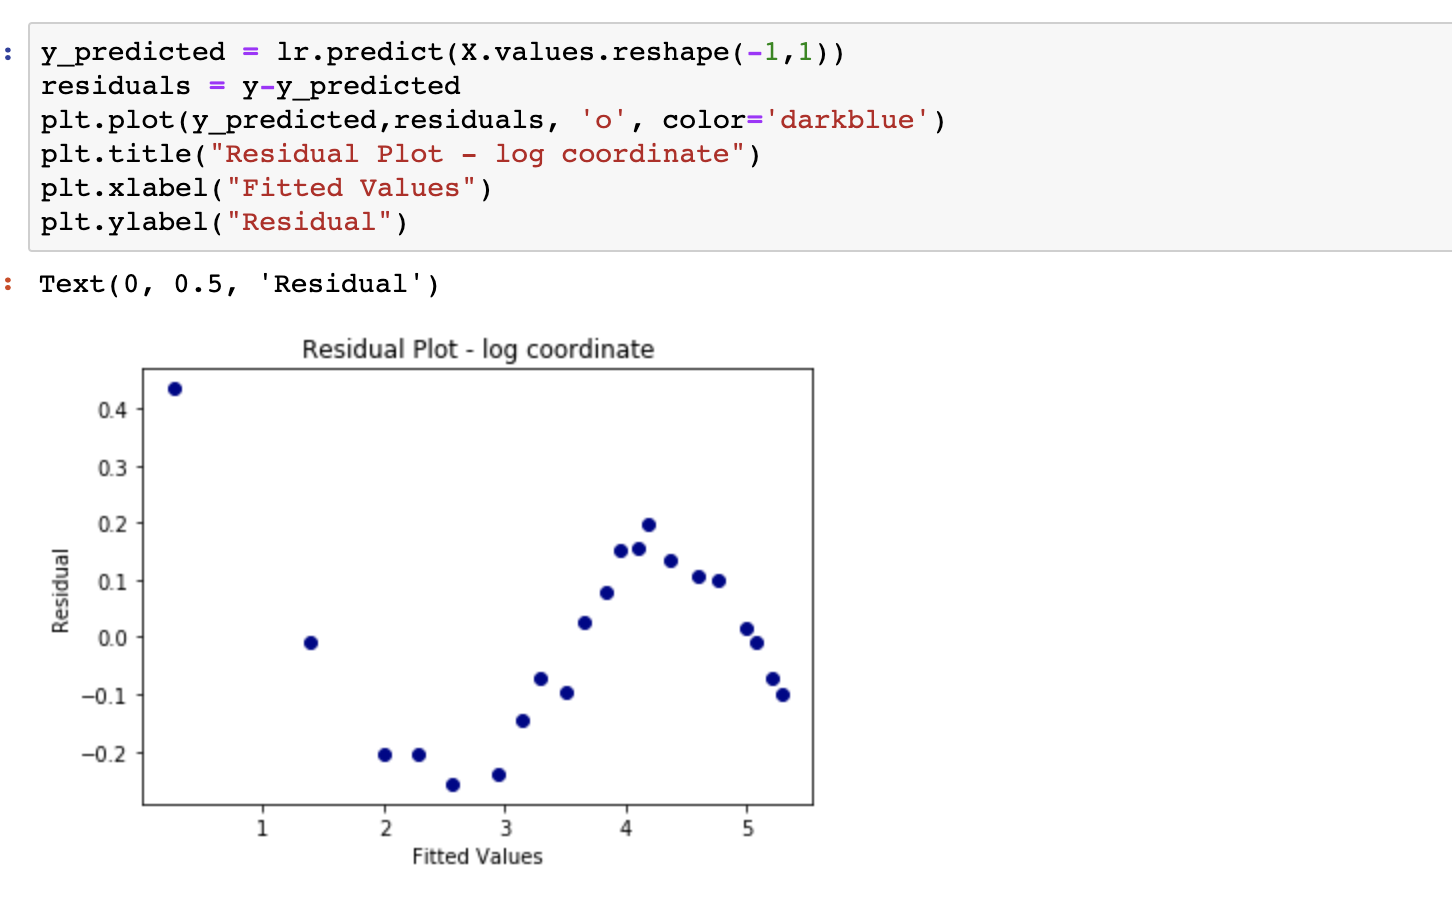
\includegraphics[width=\textwidth]{part4}
\end{figure}

Please find below the plot showing the residual against the fitted values in original coordinates

\begin{figure}[H]
\centering
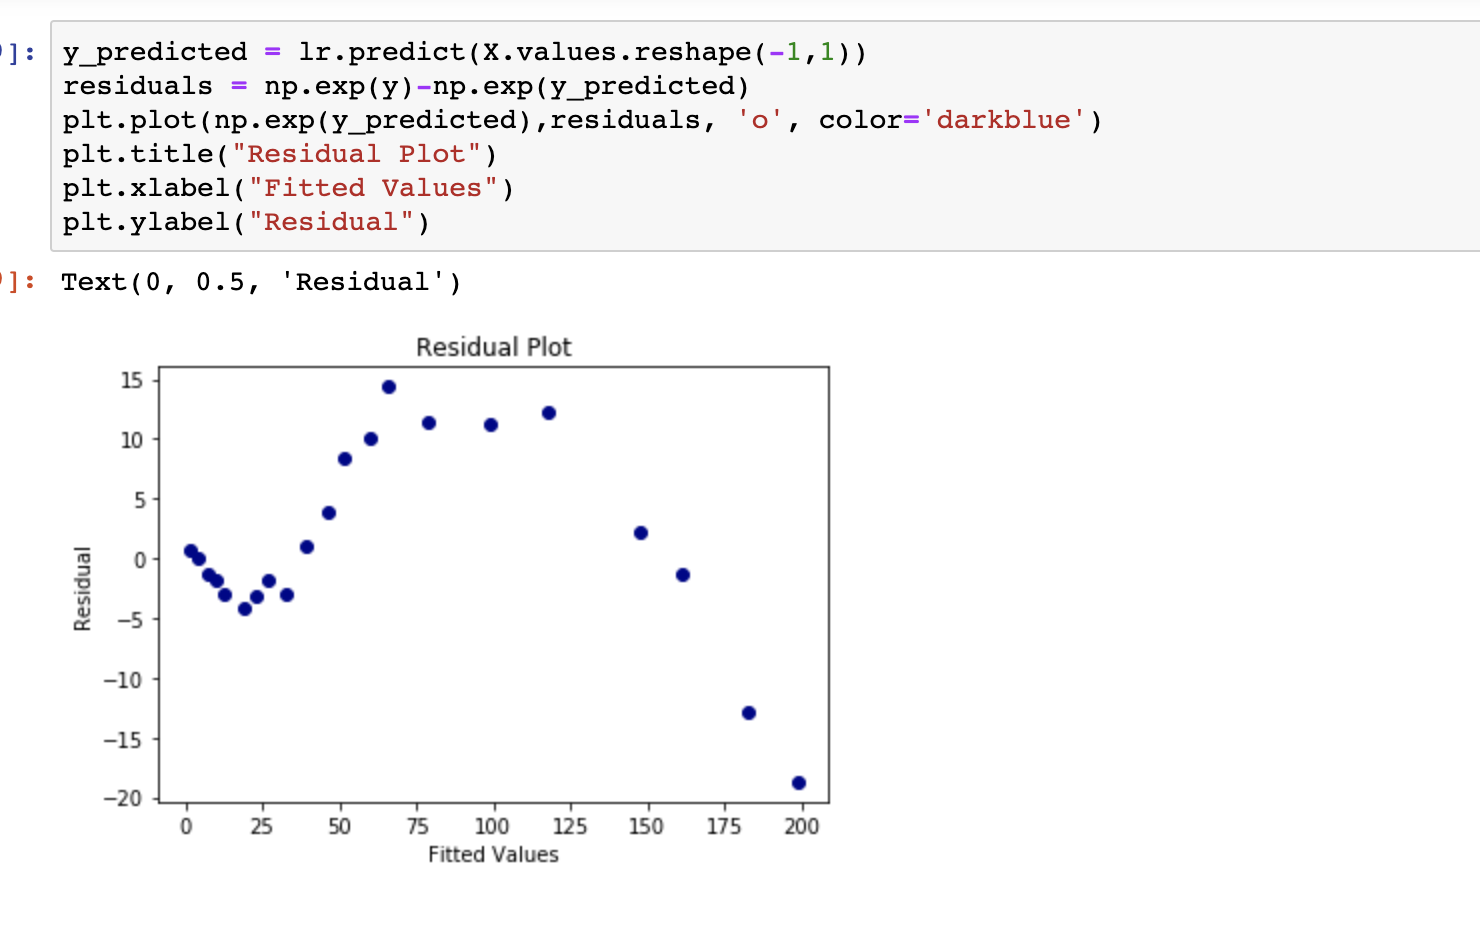
\includegraphics[width=\textwidth]{part5}
\end{figure}

\subsection{Part d} From the plot between the data points and the regressions line (Figure 1 and 2), we can observe that the predicted values are very close to the actual value. However, if we observe the residual plots (Figure 3 and 4), we understand that the model over-predicts for the first half of the data points and under-predicts for the second half of the data points. Its not very obvious from the first two figures as the residual values are low. This kind of residual plot is due to the non-linear nature of the datapoints.

\section{Problem 2} 

We built a linear regression of predicting the body mass from the diameters.

\begin{figure}[H]
\centering
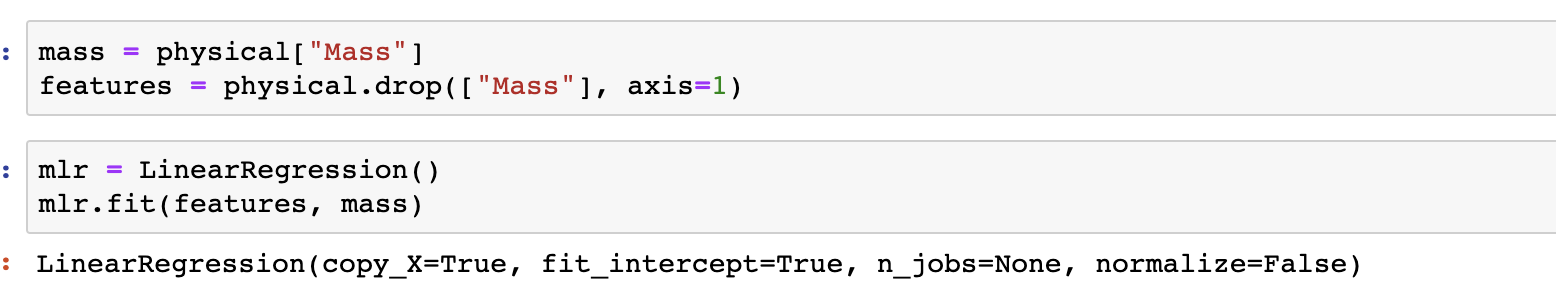
\includegraphics[width=\textwidth]{part6}
\end{figure}

\subsection{Part a}

Plot of residual against the fitted values for the regression.

\begin{figure}[H]
\centering
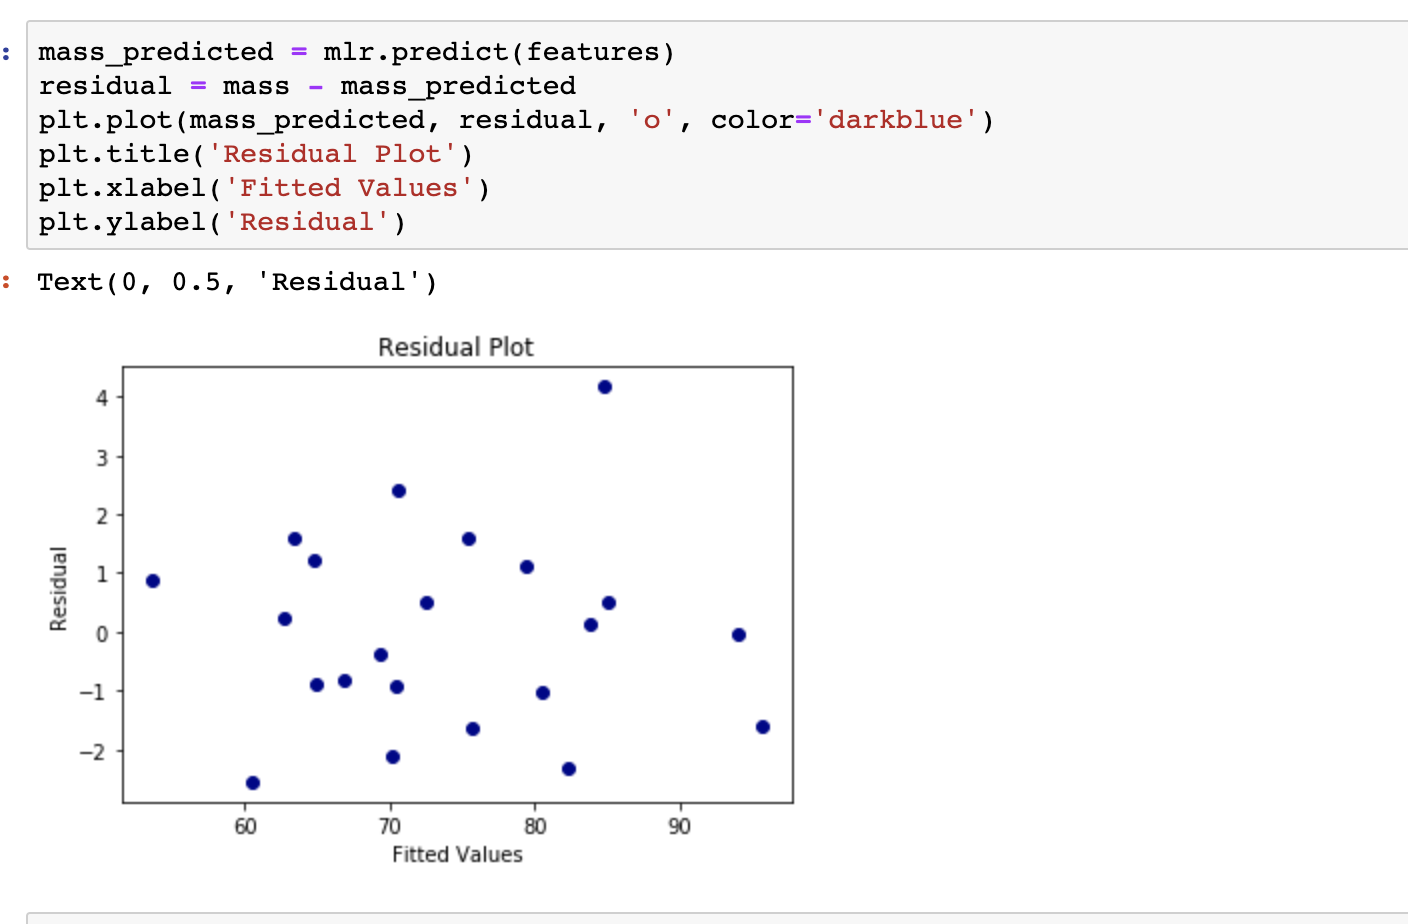
\includegraphics[width=\textwidth]{part7}
\end{figure}


\subsection{Part b}

We regressed the cube root of mass against the diameters

\begin{figure}[H]
\centering
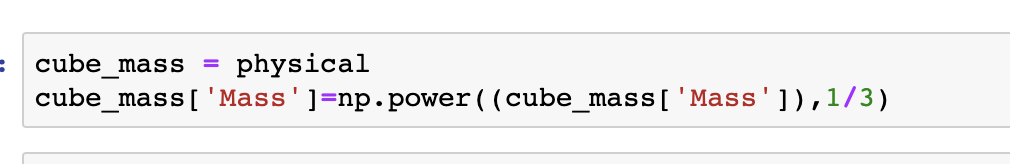
\includegraphics[width=\textwidth]{part8}
\end{figure}

Plot of residual against the fitted values for the regression.

\begin{figure}[H]
\centering
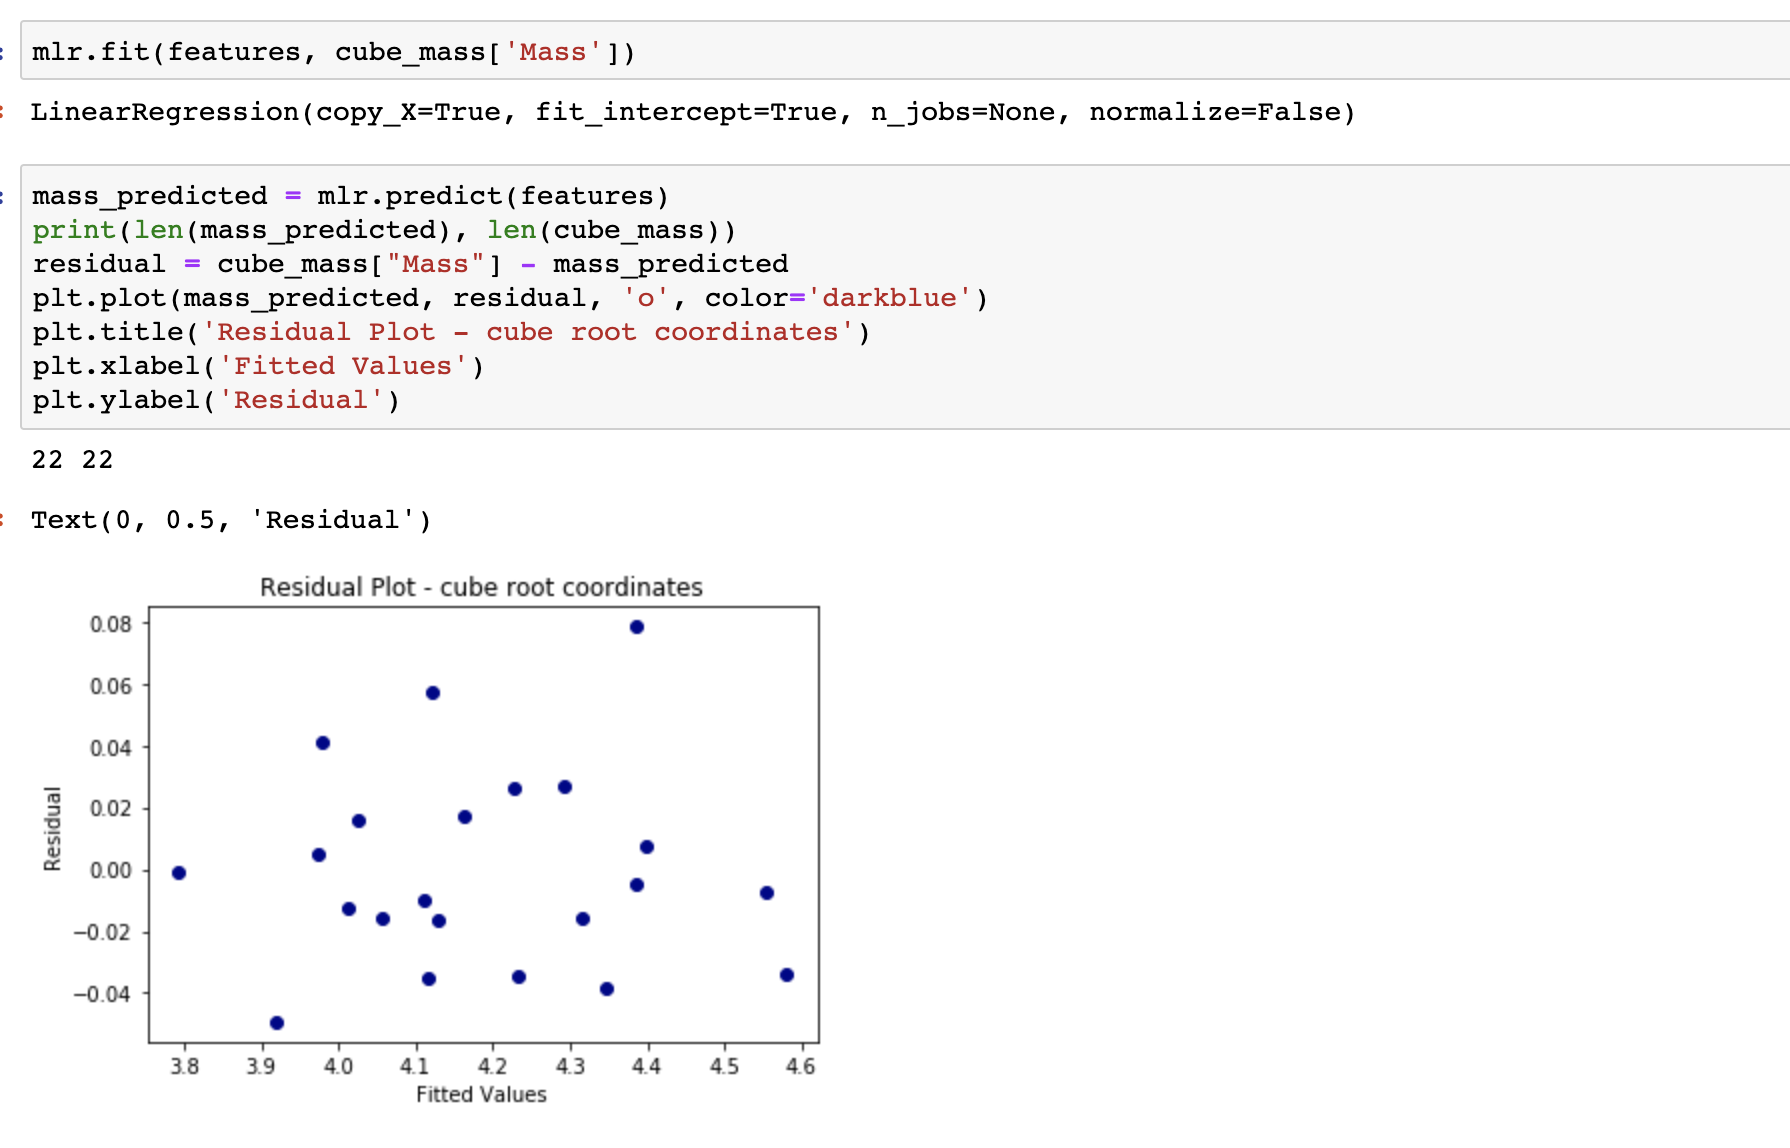
\includegraphics[width=\textwidth]{part9}
\end{figure}

\begin{figure}[H]
\centering
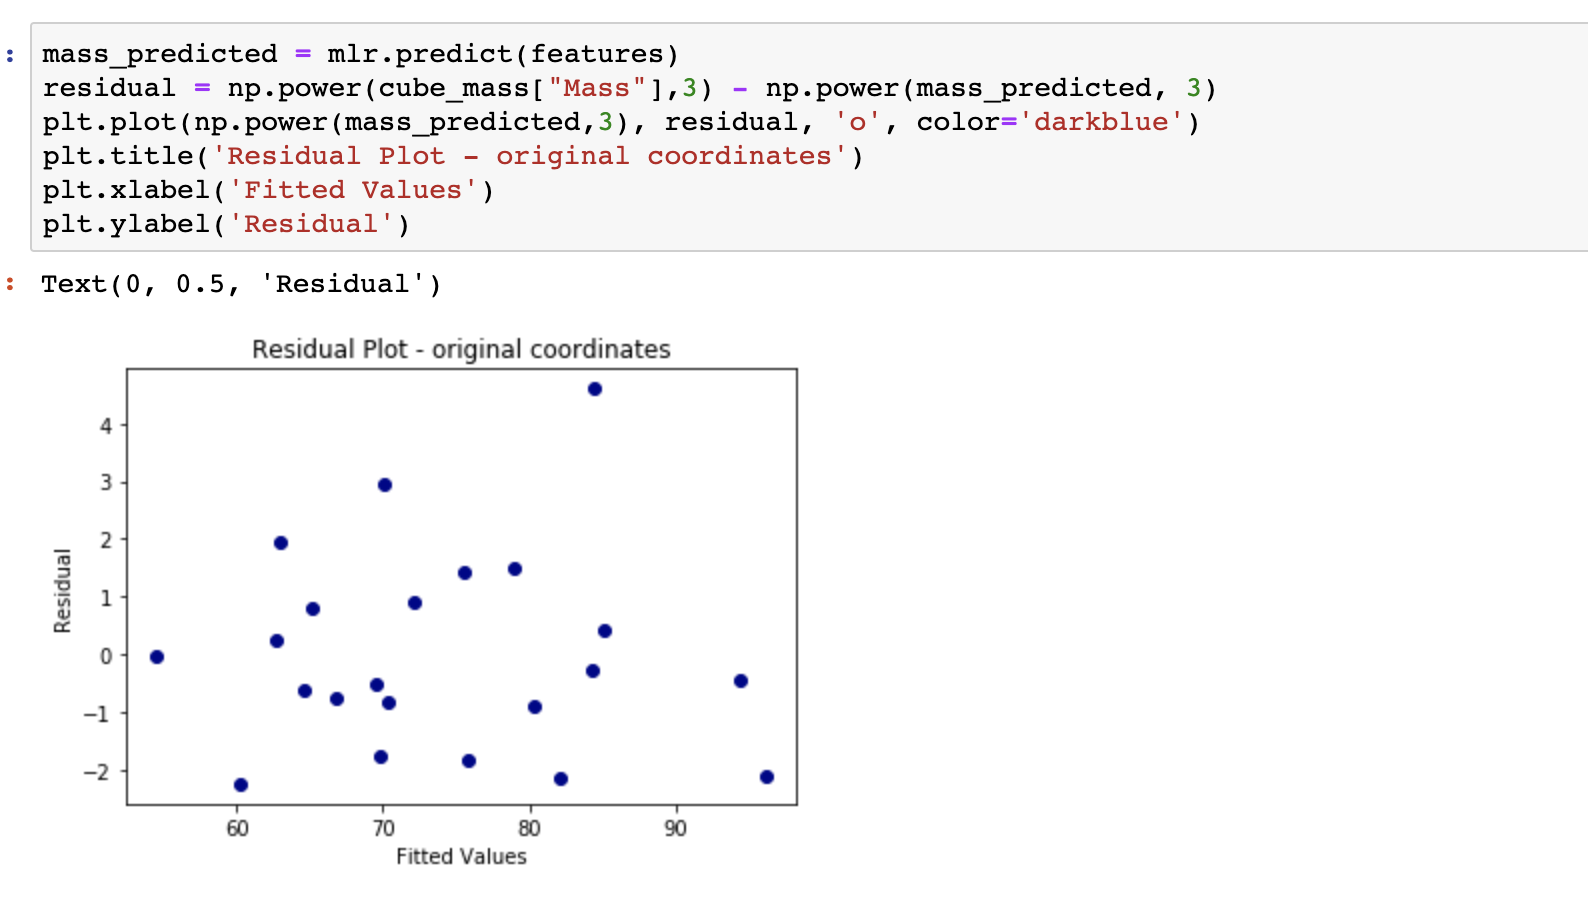
\includegraphics[width=\textwidth]{part10}
\end{figure}

\subsection{Part c} The residual plots look very identical for part a and b. The residuals are randomly distrubted around y=0 axis. Therefore, the linear regression is really good.
 
\end{document}